% from main.tex
%%%%%%%%%%  scan idx 105  |  folio 92  %%%%%%%%%%
avec \(u'v=u_X\). Pour comparer \(G_X\) et \(G'\), on peut, par exemple, former «~l'octaèdre~» de \(\Kpx(\mathcal C_X)\)
\[
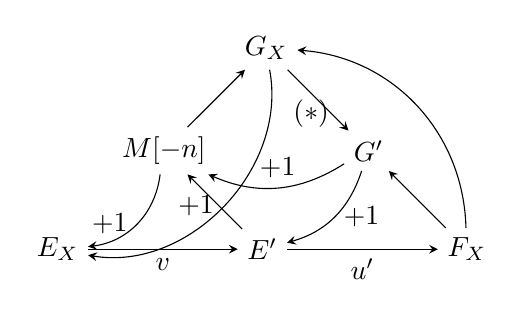
\begin{tikzpicture}[>=stealth,baseline=(GX.base),node distance=1.0cm]
  \node (EX) at (0,0) {$E_X$};
  \node (Ep) at (2.6,0) {$E'$};
  \node (FX) at (5.2,0) {$F_X$};
  \node (M)  at (1.35,1.25) {$M[-n]$};
  \node (GX) at (2.65,2.55) {$G_X$};
  \node (Gp) at (3.95,1.25) {$G'$};
  \node at (3.22,1.72) {$(*)$};
  \draw[->] (EX) -- node[below] {$v$} (Ep);
  \draw[->] (Ep) -- node[below] {$u'$} (FX);
  \draw[->] (Ep) -- (M);
  \draw[->] (M) -- (GX);
  \draw[->] (GX) -- (Gp);
  \draw[->] (FX) -- (Gp);
  \draw[->] (M) to[bend left=38] node[left] {$+1$} (EX);
  \draw[->] (Gp) to[bend left=28] node[above] {$+1$} (M);
  \draw[->] (Gp) to[bend left=28] node[right] {$+1$} (Ep);
  \draw[->] (GX) to[bend left=55] node[left] {$+1$} (EX);
  \draw[->] (FX) to[bend right=42] (GX);
\end{tikzpicture}
\]
La suite exacte de cohomologie du triangle distingué \((*)\) montre que \(\Ho^n(G_X)\longrightarrow \Ho^n(G')\) est un épimorphisme, donc que \(\Ho^n(G')\) est bien de \(\mathcal C_0\)-type fini.

La correction précédente nous ramène donc au cas où \(\Ho^{n+1}(u)\) est un monomorphisme, ce que nous supposerons maintenant. La suite exacte de cohomologie de \(E\to F\to G\) donne alors une suite exacte
\begin{equation}\tag{(.)}
  \Ho^n(E)\xrightarrow{\Ho^n(u)}
  \Ho^n(F)\longrightarrow \Ho^n(G)\longrightarrow 0.
\end{equation}
Comme \(\Ho^n(G)\) est de \(\mathcal C_0\)-type fini, l'ensemble des \(X\) au-dessus de \(S\) tels qu'il existe un épimorphisme \(M\longrightarrow \Ho^n(G_X)\) avec \(M\in\Ob\mathcal C_{0,X}\) est, par définition, un raffinement de \(S\). Utilisant la quasi-relevabilité de \(\mathcal C_0\) dans \(\mathcal C\), on peut imposer que cet épimorphisme se factorise à travers \(Z^n(F_X)\) en
\[
  M\xrightarrow{s}Z^n(F_X)\longrightarrow \Ho^n(F_X)\longrightarrow \Ho^n(G_X).
\]
Il est clair que \(u'\), défini comme en (1.4.1) avec \((r=0)\), est un morphisme de complexes et que \(\Ho^{n+1}(u')=\Ho^{n+1}(u_X)\). D'autre part, il est immédiat, à partir de la suite exacte (.), que
\[
  \Ho^n(u'):\Ho^n(E_X)\oplus M\longrightarrow \Ho^n(F_X)
\]
est un
